\chapter{Quantum Error Correction}
Quantum computers, like classical computers, suffer from \emph{noise}. That is, unwanted interactions from the outside world which causes errors in our data. For example, qubits lose their state in a very short period of time (called \emph{decoherence}). To protect against noise, there exist quantum algorithms called \emph{quantum error-correcting codes}. These algorithms encode a quantum state to make it resilient to noise. When the original state wishes to be recovered, the state can be decoded again. Applying such a code costs time and space, but gives us longer coherence times and lower error rates. To explain quantum error correction schemes, it's useful to first take a look at classical error correction.

\section{Classical Error Correction}
If you want to counter noise, you need to understand where the noise comes from. To identify a source of noise, we define a \emph{noise channel}. The most simplistic classical noise channel is the \emph{binary symmetric channel} (Figure~\ref{fig:binary_symmetric_channel}). This model assumes we have independent single-bit errors. On the left is the state of our bit. Then some time passes, after which there is a probability of $p$ that the bit has flipped due to noise, and a probability of $1 - p$ that our bit stayed in its correct state.
\begin{figure}[ht]
  \centering
  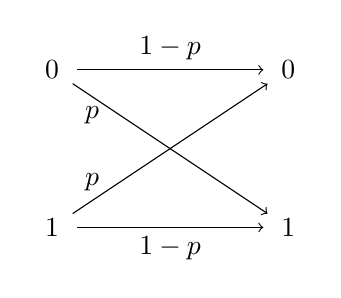
\begin{tikzpicture}
    \node (a) [circle] at (0,0) {1};
    \node (b) [circle] at (0,2) {0};
    \node (c) [circle] at (3,0) {1};
    \node (d) [circle] at (3,2) {0};
    \draw[->] (a) -- (c) node[pos=.5,below] {$1-p$};
    \draw[->] (a) -- (d) node[pos=.1,above] {$p$};
    \draw[->] (b) -- (c) node[pos=.1,below] {$p$};
    \draw[->] (b) -- (d) node[pos=.5,above] {$1-p$};
  \end{tikzpicture}
  \caption{Binary symmetric channel.}
  \label{fig:binary_symmetric_channel}
\end{figure}

A simple way to mitigate these errors is by using a repetition code, meaning we encode the message by repeating it a number of times:
\begin{align}
  0 &\rightarrow 000 \\
  1 &\rightarrow 111.
\end{align}
The bit strings $000$ and $111$ are referred to as \emph{logical} 0 and \emph{logical} 1, since they represent 0 and 1. The method of decoding is called \emph{majority voting}, which outputs the bit that appears most in the actual output. Say we want to send a bit with state $1$. We encode it with three copies as $111$. If an error occurs over the channel, for example the channel outputs $101$, majority voting gives us the correct output: $1$. When two errors occur, for example the channel outputs $001$, majority voting gives the wrong output: $0$. Majority voting with three bits fails when two errors occur, but succeeds otherwise. This code makes communication more reliable whenever $p < 1/2$.

\section{Quantum Error Correction}
We would like to develop a quantum error-correction code based on similar ideas from the classical error-correction code. However, when trying to apply these ideas to the quantum world we are faced with some difficulties:
\begin{enumerate}
  \item \emph{Measurement is destructive:} Attempting to observe the value of a quantum state by measuring it destroys the quantum state.
  \item \emph{No cloning:} Cloning a quantum state is impossible.
  \item \emph{Errors are continuous:} In the classical world, errors are discrete: a bit flip either happens or doesn't happen. With quantum states, a continuum of different errors can occur.
\end{enumerate}
As it turns out, none of these problems are fatal and quantum error-correction is possible.

We start off with looking at the noise channels: where do errors come from and how can we mitigate them. A simplistic quantum noise channel is the \emph{bit flip channel}, which is equivalent to the classical bit flip:
\begin{equation}
  \ket{\psi}\!\ket{e} \rightarrow X\ket{\psi}\!\ket{\hat{e}}.
\end{equation}
That is, the state \ket{\psi} is taken to state $X$\ket{\psi} with probability $p$, and is left in state \ket{\psi} with probability $1 - p$. Here \ket{e} is the environment and \ket{\hat{e}} the evolved environment, representing the evolution of a state and its environment. A similar noise channel is the \emph{phase flip channel}, where a state \ket{\psi} is taken to state $Z$\ket{\psi} with probability $p$, and left in state \ket{\psi} with probability $1 - p$:
\begin{equation}
  \ket{\psi}\!\ket{e} \rightarrow Z\ket{\psi}\!\ket{\hat{e}}.
\end{equation}

For simplicity sake we will only look at the bit and phase flip channels. However, these kind of errors are not very realistic. A more realistic noise channel is the \emph{amplitude dampening} or \emph{relaxation} channel. In the hardware implementation of qubits we speak of a two-state system with an excited state \ket{e} and a ground state \ket{g}, which correspond to the computational basis states \ket{1} and \ket{0}. One of these states is more energetic than the other, like in the DRAM of your computer: you charge the capacitor to represent a 1, and uncharge it to represent 0. The uncharged state 0 is very stable, it remains uncharged. The 1 state however slowly loses its charge, slowly turning into 0 state. The same goes for a two-level quantum system: the ground state \ket{g} is very stable, while the excited state \ket{e} slowly turns into the lower energetic state \ket{g}.

\subsection{Quantum Bit Flip Code}
The idea of quantum error-correction is to encode a quantum state redundantly into a larger Hilbert space. For example, we encode a single qubit $\alpha\ket{0} + \beta\ket{1}$ as $\alpha\ket{000} + \beta\ket{111}$. For convenience we write these encoded states, called \emph{code words}, as following:
\begin{align}
  \ket{0_L} &= \ket{000} \\
  \ket{1_L} &= \ket{111}.
\end{align}
We refer to \ket{0_L} and \ket{1_L} as the \emph{logical} \ket{0} and \emph{logical} \ket{1} states. This encoding is achieved by the circuit in Figure~\ref{fig:logical_encode_circ}.
\begin{figure}[ht]
  \[
    \Large
    \Qcircuit @C=1em @R=0.7em @!R {
      \push{\rule{0em}{1em}} & & \lstick{\ket{\psi}} & \ctrl{1} & \ctrl{2} & \qw \\
      \push{\rule{0em}{1em}} & & \lstick{\ket{0}} & \targ & \qw & \qw \\
      \push{\rule{0em}{1em}} & & \lstick{\ket{0}} & \qw &  \targ & \qw \\
    }
  \]
  \caption{Quantum circuit for encoding a qubit \ket{\psi} for the three qubit bit flip code.}
  \label{fig:logical_encode_circ}
\end{figure}

Suppose we encoded our state $\ket{\psi} = \alpha\ket{0} + \beta\ket{1}$ as $\ket{\psi_L} = \alpha\ket{000} + \beta\ket{111}$ and a bit flip error occurs on one qubit which we would like to correct. The first step in correcting a bit flip error is detecting if such error happened. Error detection, or \emph{syndrome diagnosis}, can be achieved through \emph{stabilizer measurements}. It is useful to make ourselves familiar with the \emph{stabilizer formalism} to understand stabilizer measurements. Consider the Bell state $\ket{\psi} = (\ket{00} + \ket{11})/\sqrt2$. This state is \emph{stabilized} by the operators $X_1X_2$ and $Z_1Z_2$, meaning $X_1X_2\ket{\psi} = \ket{\psi}$ and $Z_1Z_2\ket{\psi} = \ket{\psi}$. The basic principle behind the stabilizer formalism is that we can (often more easily) describe a state by what operators stabilize them. Stabilizers also force discrete errors, meanings all errors from all channels can be decomposed in $X$ and $Z$ errors. If we can then make an error-correction code that corrects both $X$ and $Z$ errors, we can correct \emph{any} error. Stabilizer measurements allow us to learn information about a state without fully collapsing it. We have already seen a stabilizer measurement in Section~\ref{sec:parity} to calculate the parity of a state. By calculating and measuring the parity of a state, we extracted partial information about the state without fully collapsing it.

Consider a two-qubit state $\ket{\psi} = \alpha\ket{00} + \beta\ket{11}$. We can detect what, if any, bit flip error occurred with a $Z_1Z_2$ stabilizer measurement (Figure~\ref{fig:zz_stabilizer}). The measurement result is called the \emph{error syndrome}. A $Z_1Z_2$ stabilizer measurement essentially measures the parity of the qubits \ket{d_0}\ket{d_1} using an \emph{ancilla} (helper) qubit \ket{a_0}.
\begin{figure}[ht]
  \[
    \Large
    \Qcircuit @C=1em @R=0.5em @!R {
      \push{\rule{0em}{1em}} & & & \lstick{\ket{d_0}} & \ctrl{2} & \qw & \qw & \qw \\
      \push{\rule{0em}{1em}} & & & \lstick{\ket{d_1}} & \qw & \ctrl{1} & \qw & \qw \\
      \push{\rule{0em}{1em}} & & & \lstick{\ket{a_0} = \ket{0}} & \targ &  \targ & \meter & \cw \\
    }
  \]
  \caption{Quantum circuit of a $Z_1Z_2$ stabilizer measurement.}
  \label{fig:zz_stabilizer}
\end{figure}

We can extract the error syndrome of an encoded state $\ket{\psi_L} = \alpha\ket{000} + \beta\ket{111}$ by using the two stabilizers $Z_1Z_2$ and $Z_2Z_3$ (Figure~\ref{fig:extract_error_syndrome_zz}).
\begin{figure}[ht]
  \[
    \Large
    \Qcircuit @C=1em @R=0.7em @!R {
      \push{\rule{0em}{1em}} & & & & \lstick{\ket{d_0}} & \ctrl{3} & \qw & \qw & \qw & \qw & \qw \\
      \push{\rule{0em}{1em}} & & & & \lstick{\ket{d_1}} & \qw & \ctrl{2} & \ctrl{3} & \qw & \qw & \qw \\
      \push{\rule{0em}{1em}} & & & & \lstick{\ket{d_2}} & \qw & \qw & \qw & \ctrl{2} & \qw & \qw \\
      \push{\rule{0em}{1em}} & & & & \lstick{\ket{a_0} = \ket{0}} & \targ & \targ & \qw & \qw & \meter & \cw \\
      \push{\rule{0em}{1em}} & & & & \lstick{\ket{a_1} = \ket{0}} & \qw &  \qw & \targ & \targ & \meter & \cw \\
    }
  \]
  \caption{Measuring error syndrome with stabilizer measurements $Z_1Z_2$ and $Z_2Z_3$.}
  \label{fig:extract_error_syndrome_zz}
\end{figure}

\noindent
Suppose a bit flip occurred on our encoded state \ket{\psi_L} and we're left with $\ket{\psi_L'} = \alpha\ket{001} + \beta\ket{110}$. The ancilla qubits \ket{a_0} and \ket{a_1} correspond to the stabilizer measurement of two qubits of the state:
\begin{align}
  \ket{a_0} &= Z_1Z_2\ket{\psi_L'} \\
  \ket{a_1} &= Z_2Z_3\ket{\psi_L'}.
\end{align}
For an encoded state $\alpha\ket{000} + \beta\ket{111}$ the error syndrome measurement results are both zero: $M(a_0) = M(a_1) = 0$. When this is not the case, we know we are in an erroneous state. For the state \ket{\psi_L'} we can see that
\begin{align}
  M(a_0) &= 0 \\
  M(a_1) &= 1.
\end{align}
These measurements tell us an error has occurred, and where it occurred. Assuming single bit flip errors only, an encoded state can be in one of the following states:
\begin{align}
  &\alpha\ket{000} + \beta\ket{111} \; \text{no error} \\
  X_{d_0} \rightarrow \  &\alpha\ket{100} + \beta\ket{011} \; \text{bit flip on qubit zero} \\
  X_{d_1} \rightarrow \  &\alpha\ket{010} + \beta\ket{101} \; \text{bit flip on qubit one} \\
  X_{d_2} \rightarrow \  &\alpha\ket{001} + \beta\ket{110} \; \text{bit flip on qubit two}.
\end{align}
We can find out where the error occurred by the result of the error syndrome measurement. The error syndrome measurement results corresponding to the qubit at which the error occurred can be seen in Figure~\ref{fig:zz_stabilizer_measurement_results}. To correct the state, we can simply apply an $X$ operation on the flipped qubit, flipping it back to the correct state. This error correction can be achieved through classical computing.
\begin{figure}[ht]
  \centering
  \begin{tabular}{c|c|c}
    Error & $M(a_0)$ & $M(a_1)$ \\ \hline
    None & 0 & 0 \\
    $X_{d_0}$ & 1 & 0 \\
    $X_{d_1}$ & 1 & 1 \\
    $X_{d_2}$ & 0 & 1
  \end{tabular}
  \caption{Error syndrome measurement results corresponding to where the bit flip occurred.}
  \label{fig:zz_stabilizer_measurement_results}
\end{figure}

This code can detect two errors, but only correct one. For example, consider the following erroneous states for an encoded state $\alpha\ket{000} + \beta\ket{111}$:
\begin{align}
  X_{d_0} &\rightarrow \alpha\ket{100} + \beta\ket{011} \label{eq:single_bit_flip} \\
  X_{d_1}X_{d_2} &\rightarrow \alpha\ket{011} + \beta\ket{100}. \label{eq:double_bit_flip}
\end{align}
We can detect that both states are erroneous, since for both states the error syndrome measurement results are $M(a_0) = 1$ and $M(a_1) = 0$. When correcting an erroneous state, we always choose the least amount of errors that explains the error syndrome. There's a probability of $p$ that a single error happened, and a probability of $p^2$ that two errors happened. The state in \ref{eq:double_bit_flip} would get corrected to the wrong state $\alpha\ket{111} + \beta\ket{000}$, because there's a higher probability that $X_{d_0}$ happened than $X_{d_1}X_{d_2}$. So in the case of multiple bit flip errors, corrections can be wrong and generate an unrecoverable error.

After correction we are left with an encoded state $\ket{\psi_L} = \alpha\ket{000} + \beta\ket{111}$. To get the original state $\ket{\psi} = \alpha\ket{0} + \beta\ket{1}$ back, we need to decode the state. This can be achieved by simply reversing the encoding circuit in Figure~\ref{fig:logical_encode_circ} (since \textsc{cnot} is Hermitian, the reverse of the encoding circuit is itself). Note that if you just want to do measurement, you can measure any of the qubits in $\ket{\psi_L}$ instead of decoding it.

\subsection{Quantum Phase Flip Code}
The bit flip code only catches $X$ errors. If the phase of a state \ket{\psi} flipped to $Z$\ket{\psi} and we want to correct it, we need a phase flip code. The quantum phase flip code is based on the same principles as the bit flip code. The difference with the bit flip code is that we change the basis of the state. We do this by encoding the qubits in the same way as the bit flip code, but we apply a Hadamard gate to each qubit (Figure~\ref{fig:logical_encode_circ_hadamard_basis}).
\begin{figure}[ht]
  \[
    \Large
    \Qcircuit @C=1em @R=0.7em @!R {
      \push{\rule{0em}{1em}} & & \lstick{\ket{\psi}} & \ctrl{1} & \ctrl{2} & \gate{H} & \qw \\
      \push{\rule{0em}{1em}} & & \lstick{\ket{0}} & \targ & \qw & \gate{H} & \qw \\
      \push{\rule{0em}{1em}} & & \lstick{\ket{0}} & \qw &  \targ & \gate{H} & \qw \\
    }
  \]
  \caption{Quantum circuit for encoding a qubit \ket{\psi} for the three qubit phase flip code.}
  \label{fig:logical_encode_circ_hadamard_basis}
\end{figure}
This will encode a state $\ket{\psi} = \alpha\ket{0} + \beta\ket{1}$ as $\ket{\psi_L} = \alpha\ket{+\!+\!+} + \beta\ket{-\!-\!-}$. Now when a phase flip occurs, for example $\ket{\psi_L'} = \alpha\ket{+\!-\!+} + \beta\ket{-\!+\!-}$, we can extract the error syndrome in a similar way to the bit flip code. Error syndrome measurement can be done with the stabilizers $X_1X_2$ and $X_2X_3$ as seen in Figure~\ref{fig:extract_error_syndrome_xx}. In the case of \ket{\psi_L'}, syndrome measurements are $M(a_0) = 1$ and $M(a_1) = 1$, telling us the error is in qubit \ket{d_1}. We can then correct the state by applying a $Z$ gate on \ket{d_1}. Decoding the original state is done by reversing the encoding circuit in Figure~\ref{fig:logical_encode_circ_hadamard_basis}.
\begin{figure}[ht]
  \[
    \Large
    \Qcircuit @C=1em @R=0.7em @!R {
      \push{\rule{0em}{1em}} & & & & \lstick{\ket{d_0}} & \qw & \targ & \qw & \qw & \qw & \qw & \qw & \qw \\
      \push{\rule{0em}{1em}} & & & & \lstick{\ket{d_1}} & \qw & \qw & \targ & \targ & \qw & \qw & \qw & \qw \\
      \push{\rule{0em}{1em}} & & & & \lstick{\ket{d_2}} & \qw & \qw & \qw & \qw & \targ & \qw & \qw & \qw \\
      \push{\rule{0em}{1em}} & & & & \lstick{\ket{a_0} = \ket{0}} & \gate{H} & \ctrl{-3} & \ctrl{-2} & \qw & \qw & \gate{H} & \meter & \cw \\
      \push{\rule{0em}{1em}} & & & & \lstick{\ket{a_1} = \ket{0}} & \gate{H} & \qw &  \qw & \ctrl{-3} & \ctrl{-2} & \gate{H} & \meter & \cw \\
    }
  \]
  \caption{Measuring error syndrome with stabilizer measurements $X_1X_2$ and $X_2X_3$.}
  \label{fig:extract_error_syndrome_xx}
\end{figure}

\newpage

\subsection{Shor Code}
We have seen a code which corrects bit flip and phase errors. How about a code which corrects \emph{both} errors? It turns out that this can be achieved through a \emph{concatenated} code. The \emph{Shor code} is a combination of the three qubit bit flip and phase flip code and can correct arbitrary single-qubit errors. The encoding circuit for this code can be seen in Figure~\ref{fig:encode_shor_circ}.
\begin{figure}[ht]
  \[
    \Large
    \Qcircuit @C=1em @R=0.7em @!R {
      \push{\rule{0em}{1em}} & \lstick{\ket{\psi}} & \ctrl{3} & \ctrl{6} & \gate{H} & \qw & \qw & \ctrl{1} & \ctrl{2} & \qw \\
      \push{\rule{0em}{1em}} & & & & & & \lstick{\ket{0}} & \targ & \qw & \qw \\
      \push{\rule{0em}{1em}} & & & & & & \lstick{\ket{0}} & \qw & \targ & \qw \\
      \push{\rule{0em}{1em}} & \lstick{\ket{0}} & \targ & \qw & \gate{H} & \qw & \qw & \ctrl{1} & \ctrl{2} & \qw \\
      \push{\rule{0em}{1em}} & & & & & & \lstick{\ket{0}} & \targ & \qw & \qw \\
      \push{\rule{0em}{1em}} & & & & & & \lstick{\ket{0}} & \qw & \targ & \qw \\
      \push{\rule{0em}{1em}} & \lstick{\ket{0}} & \qw &  \targ & \gate{H} & \qw & \qw & \ctrl{1} & \ctrl{2} & \qw \\
      \push{\rule{0em}{1em}} & & & & & & \lstick{\ket{0}} & \targ & \qw & \qw \\
      \push{\rule{0em}{1em}} & & & & & & \lstick{\ket{0}} & \qw & \targ & \qw
    }
  \]
  \caption{Quantum circuit for encoding a qubit \ket{\psi} for the nine qubit Shor code.}
  \label{fig:encode_shor_circ}
\end{figure}
We first apply the encode step of the phase flip code, giving
\begin{align}
  \ket{0} &\rightarrow \ket{+\!+\!+} \\
  \ket{1} &\rightarrow \ket{-\!-\!-}.
\end{align}
Then on every encoded qubit we apply the bit flip code, meaning
\begin{align}
  \ket{+} &\rightarrow \dfrac{1}{\sqrt 2}(\ket{000} + \ket{111}) \\
  \ket{-} &\rightarrow \dfrac{1}{\sqrt 2}(\ket{000} - \ket{111}).
\end{align}
This results in a nine qubit code with code words
\begin{align}
  \ket{0_L} &= \dfrac{1}{2\sqrt 2}(\ket{000} + \ket{111})(\ket{000} + \ket{111})(\ket{000} + \ket{111}) \\
  \ket{1_L} &= \dfrac{1}{2\sqrt 2}(\ket{000} - \ket{111})(\ket{000} - \ket{111})(\ket{000} - \ket{111}).
\end{align}

Error syndrome measurement for the Shor code gets a bit more hairy. The stabilizers are described in Figure~\ref{fig:shor_stabilizers}. Suppose a bit flip happens on the first qubit of a state $\ket{\psi_L} = \ket{0_L}$:
\begin{equation}
  \ket{\psi_L'} = \dfrac{1}{2\sqrt 2}(\ket{100} + \ket{011})(\ket{000} + \ket{111})(\ket{000} + \ket{111}).
\end{equation}
The stabilizer measurement $Z_1Z_2\ket{\psi_L'}$ gives us 1, so we know a bit flip occurred on the first or second qubit. Next, the stabilizer measurement $Z_2Z_3\ket{\psi_L'}$ gives us 0, so we can conclude a bit flip happened on the first qubit and we can correct it by flipping it back.
\begin{figure}[ht]
  \centering
  \begin{tabular}{c|c}
    $Z$ stabilizers & $X$ stabilizers \\ \hline
    $Z_1Z_2$ & $X_1X_2X_3X_4X_5X_6$ \\
    $Z_2Z_3$ & $X_4X_5X_6X_7X_8X_9$ \\
    $Z_4Z_5$ &  \\
    $Z_5Z_6$ &  \\
    $Z_7Z_8$ &  \\
    $Z_8Z_9$ &  \\
  \end{tabular}
  \caption{Shor code stabilizers.}
  \label{fig:shor_stabilizers}
\end{figure}

What about a phase flip? Suppose a phase flip happens on the first qubit of a state $\ket{\psi_L} = \ket{0_L}$. This phase flip flips the sign of the first block of qubits:
\begin{equation}
  \ket{\psi_L'} = \dfrac{1}{2\sqrt 2}(\ket{000} - \ket{111})(\ket{000} + \ket{111})(\ket{000} + \ket{111}).
\end{equation}
A phase flip on \emph{any} of the first three qubits has this effect, and we can correct any of these errors with the same procedure. Error syndrome measurement for a phase flip begins with comparing the phase of the first two blocks of three qubits with the stabilizer measurement $X_1X_2X_3X_4X_5X_6\ket{\psi_L'}$. The first two blocks $(\ket{000} - \ket{111})(\ket{000} + \ket{111})$ have different signs, and the stabilizer measurement will measure 1. The second two blocks $(\ket{000} + \ket{111})(\ket{000} + \ket{111})$ have equal signs, and the stabilizer measurement $X_4X_5X_6X_7X_8X_9\ket{\psi_L'}$ measures 0. We can conclude that the phase flipped in the first block of three qubits and we can correct it by flipping the sign of the first block. These methods to correct errors will work for any of the nine qubits.

To describe more complex circuits it's useful to adopt a shorthand notation:
\[
  \Large
  \Qcircuit @C=1em @R=0.7em @!R {
    & & \ctrl{1} & \qw & & & \ctrl{1} & \ctrl{2} & \qw \\
    & & \gate{U} & \qw & = & & \gate{U} & \qw & \qw \\
    & & \gate{U} \qwx & \qw & & & \qw & \gate{U} & \qw
  }
\]
We can then describe the error syndrome measurement circuit of the Shor code as seen in Figure~\ref{fig:shor_esm_circ}.

\newpage

\begin{figure}[!ht]
  \[
    \large
    \Qcircuit @C=0.9em @R=0.7em @!R {
      \push{\rule{0em}{1em}} & & & & \lstick{\ket{d_0}} & \qw & \gate{Z} & \qw & \qw & \qw & \qw & \qw & \gate{X} & \qw & \qw & \qw \\
      \push{\rule{0em}{1em}} & & & & \lstick{\ket{d_1}} & \qw & \gate{Z} \qwx & \gate{Z} & \qw & \qw & \qw & \qw & \gate{X} \qwx & \qw & \qw & \qw \\
      \push{\rule{0em}{1em}} & & & & \lstick{\ket{d_2}} & \qw & \qw & \gate{Z} \qwx & \qw & \qw & \qw & \qw & \gate{X} \qwx & \qw & \qw & \qw \\
      \push{\rule{0em}{1em}} & & & & \lstick{\ket{d_3}} & \qw & \qw & \qw & \gate{Z} & \qw & \qw & \qw & \gate{X} \qwx & \gate{X} & \qw & \qw \\
      \push{\rule{0em}{1em}} & & & & \lstick{\ket{d_4}} & \qw & \qw & \qw & \gate{Z} \qwx & \gate{Z} & \qw & \qw & \gate{X} \qwx & \gate{X} \qwx & \qw & \qw \\
      \push{\rule{0em}{1em}} & & & & \lstick{\ket{d_5}} & \qw & \qw & \qw & \qw & \gate{Z} \qwx & \qw & \qw & \gate{X} \qwx & \gate{X} \qwx & \qw & \qw \\
      \push{\rule{0em}{1em}} & & & & \lstick{\ket{d_6}} & \qw & \qw & \qw & \qw & \qw & \gate{Z} & \qw & \qw & \gate{X} \qwx{-1} & \qw & \qw \\
      \push{\rule{0em}{1em}} & & & & \lstick{\ket{d_7}} & \qw & \qw & \qw & \qw & \qw & \gate{Z} \qwx{-1} & \gate{Z} & \qw & \gate{X} \qwx{-1} & \qw & \qw \\
      \push{\rule{0em}{1em}} & & & & \lstick{\ket{d_8}} & \qw & \qw & \qw & \qw & \qw & \qw & \gate{Z} \qwx{-1} & \qw & \gate{X} \qwx{-1} & \qw & \qw \\
      \push{\rule{0em}{1em}} & & & & \lstick{\ket{a_0} = \ket{0}} & \gate{H} & \ctrl{-8} & \qw & \qw & \qw & \qw & \qw & \qw & \qw & \gate{H} & \qw \\
      \push{\rule{0em}{1em}} & & & & \lstick{\ket{a_1} = \ket{0}} & \gate{H} & \qw & \ctrl{-8} & \qw & \qw & \qw & \qw & \qw & \qw & \gate{H} & \qw \\
      \push{\rule{0em}{1em}} & & & & \lstick{\ket{a_2} = \ket{0}} & \gate{H} & \qw & \qw & \ctrl{-7} & \qw & \qw & \qw & \qw & \qw & \gate{H} & \qw \\
      \push{\rule{0em}{1em}} & & & & \lstick{\ket{a_3} = \ket{0}} & \gate{H} & \qw & \qw & \qw & \ctrl{-7} & \qw & \qw & \qw & \qw & \gate{H} & \qw \\
      \push{\rule{0em}{1em}} & & & & \lstick{\ket{a_4} = \ket{0}} & \gate{H} & \qw & \qw & \qw & \qw & \ctrl{-6} & \qw & \qw & \qw & \gate{H} & \qw \\
      \push{\rule{0em}{1em}} & & & & \lstick{\ket{a_5} = \ket{0}} & \gate{H} & \qw & \qw & \qw & \qw & \qw & \ctrl{-6} & \qw & \qw & \gate{H} & \qw \\
      \push{\rule{0em}{1em}} & & & & \lstick{\ket{a_6} = \ket{0}} & \gate{H} & \qw & \qw & \qw & \qw & \qw & \qw & \ctrl{-10} & \qw & \gate{H} & \qw \\
      \push{\rule{0em}{1em}} & & & & \lstick{\ket{a_7} = \ket{0}} & \gate{H} & \qw & \qw & \qw & \qw & \qw & \qw & \qw & \ctrl{-8} & \gate{H} & \qw \\
    }
  \]
  \caption{Error syndrome measurement circuit for the nine qubit Shor code.}
  \label{fig:shor_esm_circ}
\end{figure}

\newpage

\subsection{Steane Code}
The Shor code was the first complete quantum error-correction code presented, but it is not the most efficient. The \emph{Steane code} is a seven qubit error-correction code which can correct arbitrary single-qubit errors. It turns out that the most efficient complete quantum error-correction code can be achieved with five qubits, but we will look at the Steane code because it's mathematically very convenient. The Steane code encode circuit is described in Figure~\ref{fig:steane_enc_circ}, and gives the following code words:
\begin{gather}
  \begin{aligned}
    \ket{0_L} = \dfrac{1}{\sqrt8}\Big(&\ket{0000000} + \ket{1010101} + \ket{0110011} + \ket{1100110} \\
    + \, &\ket{0001111} + \ket{1011010} + \ket{0111100} + \ket{1101001} \Big)
  \end{aligned} \\
  \begin{aligned}
    \ket{1_L} = \dfrac{1}{\sqrt8}\Big(&\ket{1111111} + \ket{0101010} + \ket{1001100} + \ket{0011001} \\
    + \, &\ket{1110000} + \ket{0100101} + \ket{1000011} + \ket{0010110} \Big).
  \end{aligned}
\end{gather}

\noindent
Error syndrome measurement is achieved in a similar way as the Shor code, but with six ancilla qubits and different stabilizers. The stabilizers used in error syndrome measurement can be found in Figure~\ref{fig:steane_stabilizers}.
\begin{figure}[ht]
  \begin{minipage}{.59\textwidth}
    \[
      \Large
      \Qcircuit @C=1.1em @R=0.7em @!R {
        \push{\rule{0em}{1em}} & \lstick{\ket{\psi}} & \ctrl{1} & \qw & \gate{X} & \gate{X} & \qw \\
        \push{\rule{0em}{1em}} & \lstick{\ket{0}} & \gate{X} & \gate{X} & \qw \qwx & \gate{X} \qwx & \qw \\
        \push{\rule{0em}{1em}} & \lstick{\ket{0}} & \gate{X} \qwx & \gate{X} \qwx & \gate{X} \qwx & \qw \qwx & \qw \\
        \push{\rule{0em}{1em}} & \lstick{\ket{0}} & \qw & \gate{X} \qwx & \gate{X} \qwx & \gate{X} \qwx & \qw \\
        \push{\rule{0em}{1em}} & \lstick{\ket{0}} & \gate{H} & \ctrl{-1} & \qw & \qw & \qw \\
        \push{\rule{0em}{1em}} & \lstick{\ket{0}} & \gate{H} & \qw & \ctrl{-2} & \qw & \qw \\
        \push{\rule{0em}{1em}} & \lstick{\ket{0}} & \gate{H} & \qw & \qw & \ctrl{-3} & \qw
      }
    \]
    \caption{Quantum circuit for encoding a qubit \ket{\psi} for the seven qubit Steane code.}
    \label{fig:steane_enc_circ}
  \end{minipage}%
  \hspace*{.01\textwidth}
  \begin{minipage}{.4\textwidth}
    \centering
    \begin{tabular}{c|c}
      $Z$ stabilizers & $X$ stabilizers \\ \hline
      $Z_1Z_3Z_5Z_7$ & $X_1X_3X_5X_7$ \\
      $Z_2Z_3Z_6Z_7$ & $X_2X_3X_6X_7$ \\
      $Z_4Z_5Z_6Z_7$ & $X_4X_5X_6X_7$
    \end{tabular}
    \caption{Steane code stabilizers.}
    \label{fig:steane_stabilizers}
  \end{minipage}
\end{figure}

\section{Towards Fault-tolerant Universal Quantum Computing}
In Section~\ref{sec:universal_gate_sets} we briefly discussed universal quantum computing. Universal quantum computing can be achieved through universal gate sets consisting of the complete Clifford set and one or more non-Clifford gates. We have seen how we can use quantum error-correction codes to mitigate errors from noise. \emph{Fault tolerance} means that we can not only mitigate and fix some of these errors, but that we can contain these errors. That is, if an error occurs it doesn't spread out and infect your whole system with errors. So when we talk about fault-tolerant universal quantum computing, we talk about being able to do computation in a universal way, and also being able to contain and correct errors.

In order to achieve fault-tolerant universal quantum computing, we need to be able to perform logical operations on our encoded logical qubits. To do useful computation, we also need the ability of multiple logical qubits. So far we have only looked at single logical qubits. Furthermore, errors can occur on the ancillary qubits and inject errors into the data qubits, which we need to be resistant to. These are some of the problems we need to overcome to achieve fault-tolerant universal quantum computing.
